\section{Computational Experiments}
We develop a prototype scheduling system based on the described improved genetic algorithm and validate its performance based on testing instances.
Since there exist no benchmark instances in the literature specifically designed for dynamic scheduling problems, we create testing instances based on the widely used FT20 problem and add dynamic data when dynamic scheduling is required.
These testing instances are then used to simulate the scheduling problems in dynamic manufacturing environments where unexpected events and urgent jobs arrivals happen often.
In the experiment, minimization of mean flow time is used as the objective function in the case of unexpected events; a multi-objective of minimizing maximal make-span and total tardiness is used as the objective function in the case of urgent job insertion.

Parameters of the improved genetic algorithm are set as follows: population size $P = 200$; crossover probability $P_c = 0.8$; crossover times $n = 10$; mutation probability $P_m = 0.01$ and total number of iterations as 100.
Figure \ref{fig:fig2} shows the initial scheduling plan for the FT20 instance with 20 jobs to be processed on 5 machines.
This initial plan represents the solution for this problem and the maximum completion time is 1165.

\begin{figure}[h!]
	\begin{center}
		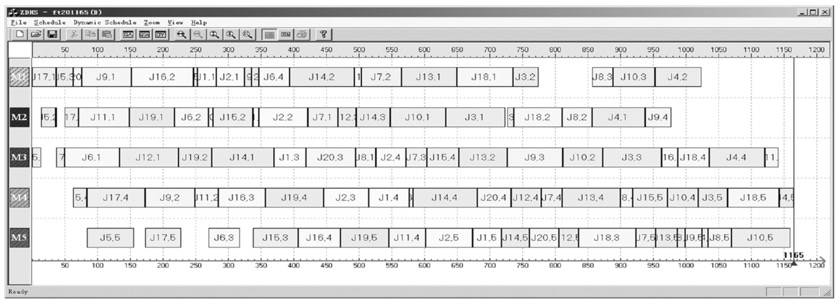
\includegraphics[width=1\linewidth]{sections/figure2.jpg}
		\caption{Initial scheduling plan}
		\label{fig:fig2}
	\end{center}
\end{figure}


Suppose the following stochastic events happen at time 600: 1) processing time of job $(J_{10}, 1)$ on machine 2 is delayed for 30 time units, due to machine breakdown, work delay or other reasons; 2) jobs $(J_1, 3)$ and $(J_{20}, 3)$ on machine 3 are exchanged due to worker absenteeism or vacation; 3) starting time of job $(J_8, 1)$ on machine 3 is delayed for 60 time units due to delayed arrival of raw materials; 4) starting time of job $(J_{11}, 4)$ on machine 5 is delayed for 40 time units due to delayed assembly;
The maximal completion time is delayed to 1219 after the manual adjustments to accommodate the above random events.
The improved genetic algorithm is applied at time 600 to reschedule the updated jobs and figure \ref{fig:fig3} shows the optimal schedule of this scenario and the maximal completion time is reduced to 1202.


\begin{figure}[h!]
	\begin{center}
		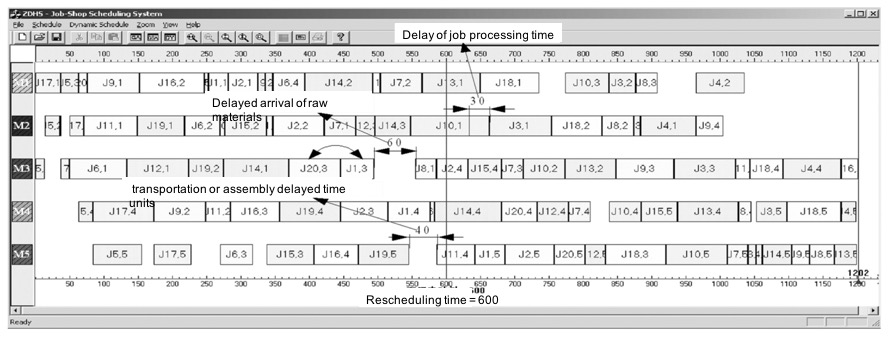
\includegraphics[width=1\linewidth]{sections/figure3.jpg}
		\caption{Event-driven rescheduling plan}
		\label{fig:fig3}
	\end{center}
\end{figure}


To further validate the performance of rolling horizon optimization strategy, we assume the arrival of urgent jobs at time 600 in addition to the aforementioned stochastic events.
There are three jobs in the urgent arrivals, namely, job 21, 22 and 23, and they are required to finish before given delivery due date.
Table \ref{tab:tab1} gives the processing machines, processing times, release times and delivery due dates of the three jobs.
Note that delivery due dates are defined by multiplying average processing time by 1.8 and adding the results to the rescheduling time point of 600.
In this scenario, the scheduled jobs need to be processed as soon as possible, while new urgent jobs must be finished before delivery due date.
To this purpose, we need to solve the multi-objective dynamic scheduling problem considering both maximal job completion time and total tardiness. 
Using this multi-objective function, the improved genetic algorithm is used to reschedule all the jobs at time 600 and figure \ref{fig:fig4} shows the optimal solution.
It can be seen from the figure that all the three newly inserted jobs are finished processing before time 900 and the maximal completion time is 1338.


\begin{table}[h!]
	\begin{center}
		\caption{Processing machine, processing time and release time for each urgent job}
		\label{tab:tab1}
		\begin{tabular}{cccccccc}
			\hline
			\multirow{2}{*}{job} & \multicolumn{5}{c}{processing machine/time} & release time & delivery due time \\
			\cline{2-6}
			& 1 & 2 & 3 & 4 & 5 & & \\
			\hline 
			job 21 & 1(29) & 2(9) & 3(49) & 4(12) & 5(26) & 650 & 900\\
			job 22 & 3(18) & 2(22) & 1(36) & 4(21) & 5(72) & 600 & 900 \\
			job 23 & 2(46) & 1(28) & 3(32) & 5(40) & 4(30) & 680 & 900 \\
			\hline
		\end{tabular}
	\end{center}
\end{table}




\begin{figure}[h!]
	\begin{center}
		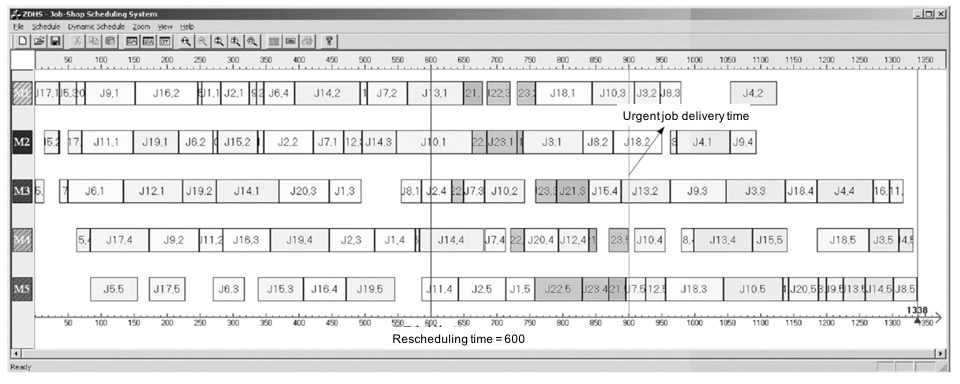
\includegraphics[width=1\linewidth]{sections/figure4.jpg}
		\caption{Multi-objective dynamic scheduling plan after insertion of urgent jobs}
		\label{fig:fig4}
	\end{center}
\end{figure}

The above rescheduling strategy can be used together with the improved genetic algorithm to continuously optimize all the jobs within a rolling horizon.
The computational results show that a complex dynamic scheduling problem can be naturally divided into multiple scheduling horizons and static scheduling algorithm can then be used to optimize job schedules within each horizon, which improves the scheduling capability in adapting to dynamically changing manufacturing environments and urgent events and jobs can be tackled promptly.
This strategy can be used in other dynamic scheduling problems as well.